\documentclass[10pt,a4paper]{article}
\usepackage{graphicx} %LaTeX package to import graphics
\graphicspath{image/} %configuring the graphicx package,le immagini si trovano in image/
\usepackage{float}
\usepackage[utf8]{inputenc}
\usepackage[T1]{fontenc}
\title{Ambliopia}
\author{Luca Frangiamore}

\date{2023}

\begin{document}
	
	\maketitle
	\tableofcontents{\tiny }
	
	
	\begin{abstract}
		Trattazione condizione dell'ambliopia anche detta "occhio pigro" mediante l'utilizzo di un applicativo mobile.
	\end{abstract}
	 \newpage
	\section {Ambliopia}
	L'ambliopia, anche conosciuta come "occhio pigro" è una patologia che si manifesta nei prima anni dello sviluppo, età compresa tra 0-6 anni, il quale colpisce circa il 4\% della popolazione mondiale.
	La patologia riguarda la non corretta stimolazione dell'apparato visivo, in questo caso il cervello non riesce a ricreare l'immagine tridimensionale e quindi per evitare il fenomeno della visione doppia, anche detta \textbf{diplopia}, il cervello tenterà a sopprimere un immagine.
	Nella maggior parte dei casi, l'occhio è anatomicamente perfetto, \textbf{ambliopia funzionale}, in casi peggiori possiamo riscontrare \textbf{ambliopia organica} in cui vi è una deviazione delle vie ottiche.
	La seguente patologia si può manifestare con più probabilità in maniera asimmetrica, \textbf{monolaterale}, il quale colpisce un solo occhio o più raramente possiamo trovare la forma \textbf{bilaterale}, il quale colpisce entrambi gli occhi.
	Normalmente l'ambliopia non peggiora durante la vita adulta in quanto oramai lo sviluppo alterato della vista si è oramai instaurato, l'età in cui l'ambliopia si stabilizzi in modo permanente va dagli 8 ai 15 anni.
	\subsection{Diagnosi}
	\begin{itemize}
		\item Classica, in cui il medico cerca di stabilire l'acuità visiva e la visione binoculare del piccolo paziente. In caso di strabismo sarà necessaria anche una visita ortottica.
		\item Pediatric Vision Scanner, Negli ultimi anni si sta sviluppando un nuovo metodo in grado di riconoscere l'ambliopia in età pediatrica con alta precisione.
		Come pubblicato nel articolo 	ARTICOLOOOOO, in cui si prende in esame Pediatric Vision Scanner(PVS), si è riscontrata una precisione del 100\%, ovvero tutti e 6 i bambini sono stati identificati correttamente.
		Il seguente metodo potrebbe permettere di diagnosticare l'ambliopia già dai 2 di età.
		\begin{figure}[h]
			\centering
			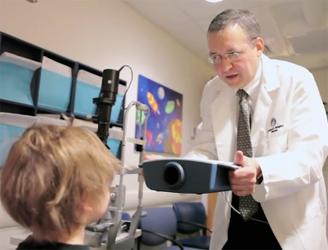
\includegraphics[width=0.6\linewidth]{image/pvs}
			\caption{Pediatric Vision Scanner}
			\label{fig:pvs}
		\end{figure}
	\end{itemize}
	\subsection{Cause}
	In generale come detto prima, l'occhio pigro riguarda il progressivo trascuramento dei segnali di uno dei due occhi.
	Questo processo di sviluppo è causato da un non corretto sviluppo delle vie nervose degli occhi, le quali vengono stimolate in modo non bilanciate, ciò è dovuto magari dalla presenza di una condizione oculare presente in uno dei due occhio(nel caso di \textbf{monolaterale }.
	Alcune condizioni che possono insorgere sono:
	\begin{itemize}
		\item Astigmatismo:Visione è poco nitida e distorta in qualsivoglia direzione.
		\item Strabismo:Deviazione degli assi visivi, impedisce il corretto coordinamento degli occhi. 
		\item Cataratta:Opacizzazione parziale o totale del cristallino,  causa offuscamento e difficoltà nel mettere a fuoco le immagini.
		\item Ptosi palpebrale:Una o entrambi le palpebre sono superiori sono abbassate più del normale.
	\end{itemize}
	Come detto prima, se il cervello non riesce a combinare le immagini proveniente dai due occhi, esso può decidere di trascurare un dei due segnali, prediligendo l'occhio ottimale, sviluppando quindi l'ambliopia.
	\subsection{Sintomi}
	Vi sono alcuni casi, in cui il paziente probabilmente giovane, non si accorge della patologia, questo può ritardare o eliminare i trattamenti attui a ridurre o eliminare il problema.
	Tra i problemi più comuni possiamo citare:	   
	\begin{itemize}
		\item Difficoltà dei visione in un occhio.
		\item Movimenti involontari dell'occhio.
		\item Sensibilità al movimento compromessa.
		\item Scarsa percezione della profondità in quanto il cervello privilegia un occhio a causa della ridotta acuità visiva dell'altro.
	\end{itemize} 
\newpage   
	\subsection{Trattamenti}
	Subito dopo aver riconosciuto il disturbo bisogna procedere con la corretto terapia. Per prima cosa si corregge il difetto che ha portato l'inibizione dell'occhio pigro, successivamente si procede con la terapia occlusiva permette di stimolare l'occhio pigro in modo da costringerlo a lavorare.
	\begin{itemize}
		\item Patching, La terapia consiste nel coprire l'occhio dominante, da applicare per un perioda di tempo variabile.
		Il trattamento è efficacie ma il recupero della vista impiega diversi mesi.       	   
			\begin{figure}[h]
				\centering
				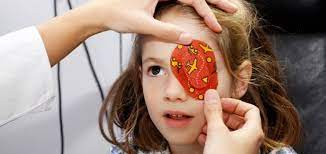
\includegraphics[width=0.7\linewidth]{image/patching}
				\caption{Trattamento con Patching}
				\label{fig:patching}
			\end{figure}	
	
		\item Penalizzazione ottica, consiste nel indossare dei supporti fisici, con delle lenti con diversi gradi di opacizzazione.
		
			\begin{figure}[h]
				\centering
				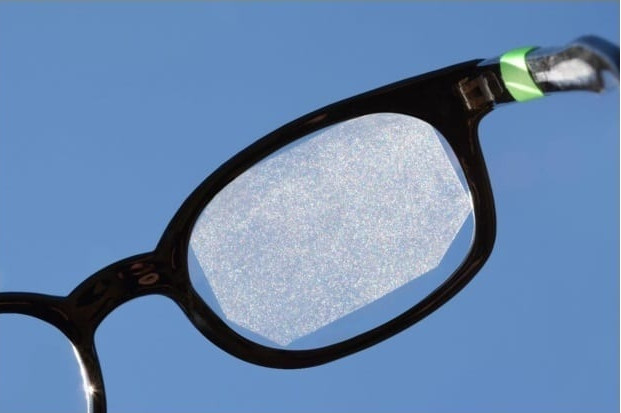
\includegraphics[width=0.7\linewidth]{image/penalizzazione ottica}
				\caption{Trattamento con lente di bangerter}
				\label{fig:penalizzazione-ottica}
			\end{figure}
    	\newpage
		\item Collirio, permette di offuscare la vista dell'occhio dominante, in modo da poter stimolare il l'occhio più debole
		
		\item Luminopia, è un software approvato da  \textbf{Food and Drug Administration(FDA)} come annunciato dal CEO Scott Xiao, che permette ai pazienti di poter usufruire di 700 ore di serie o film, adattati tramite AI, questo permette di rendere il trattamento dell'ambliopia piacevole e quindi sopportabile nel lungo periodo.
		I pazienti usufruiscono di questi contenuti mediante il vr, in modo da poter visionare i contenuti scelti.
			\begin{figure}[h]
				\centering
				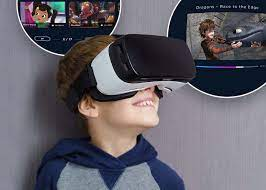
\includegraphics[width=0.7\linewidth]{image/luminopia}
				\caption{Trattamento innovativo con Luminopia}
				\label{fig:luminopia}
			\end{figure}
	\end{itemize}
	Maggiore è l'età della diagnosi, minori sono le possibilità di recupero dall'ambliopia.\\
	\newpage
	\section{3D4Amb}
	Il progetto è nato con l'intenzione di, creare uno strumento utile ed economico per il trattamento dell'occhio pigro basato sul 3D e per andare a misurare l'ambliopia.
	
	\subsection{Funzionamento}
	Il funzionamento di base è sempre lo stesso, si va a mostrare al paziente due immagini diverse ma correlate tra loro, pre-elaborate tramite il software 3D4Amb.
	3D4Amb utilizza diversi supporti tecnologici, come il cardboard o la il quale ci permette di realizzare delle applicazione video ludiche basate sulla differenziazione delle immagini,come detto sopra, il tutto relativamente a basso costo.
	Per poter utilizzare 3D4Amb bisogna garantire lo sdoppiamento delle immagine per i due occhi, le quali dovranno essere mostrate ai due occhi, per garantire la corretta esposizione si sono sperimentate diverse strade tra cui, Cardboard o occhiali anaglifici.
	\subsubsection{Cardboard}
	Questo dispositivo ci permette di poter usufruire della tecnolagia 3D con un costo relativamente basso che si aggira sui 10\$, esso ci permette di mostrare/alterare alcuni elementi i una delle due lenti, in cui si trova l'occhio sano. 
	\begin{figure}[H]
		\centering
		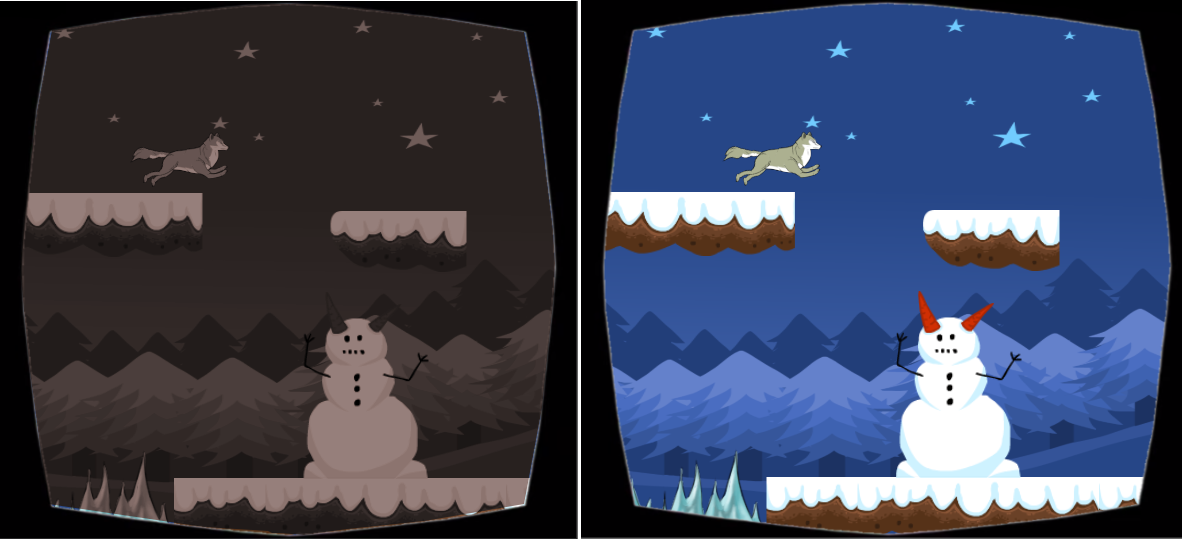
\includegraphics[width=0.7\linewidth]{image/3D4Amb}
		\caption{Gioco creato per il cardboard }
		\label{fig:cardboard-3D4Amb}
	\end{figure}
    Come mostrato nella figura \label{cardboard-3D4Amb}, le immagini mostrate differisco per il colore, vi sono casi in cui si può andare ad mettere un elemento della scena
	\subsubsection{Occhiali Anaglifici}
	\subsection{Obiettivi}
	Utilizzando la tecnologia 3D è possibile trattare la l'ambliopia, attraverso un approccio ludico, permettendo quindi di intrattenere maggiormente il paziente, spesso in età giovanile, aumentando quindi la probabilità di successo.
	I punti in cui 3D4Amb si focalizza sono:
	\begin{itemize}
		\item Basso costoso, il sistema e si basa su tecnologie a basso costo.
		\item Facile da usare, non richiede nessun particolare capacità, permettendo anche ai pazienti più piccoli di poter usufruire del sistema senza l'assistenza dei genitori.
		\item Uso domestico, il sistema può essere utilizzato nel ambiente domestico, evitando quindi le visite frequenti all'ospedale
		\item Facilmente estendibile, 3D4Amb permette di usare le librerie software, agevolando  quindi l'estensione del sistema, aggiungendo nuove applicazione o funzioni.
	\end{itemize}
	
	\section{title}
	\thanks{Cristina D'avena,Matteo Verzeroli }
\end{document}